\documentclass{beamer}
%
% Choose how your presentation looks.
%
% For more themes, color themes and font themes, see:
% http://deic.uab.es/~iblanes/beamer_gallery/index_by_theme.html
%
\mode<presentation>
{
  \usetheme{Madrid}      % or try Darmstadt, Madrid, Warsaw, ...
  \usecolortheme{beaver} % or try albatross, beaver, crane, ...
  \usefonttheme{serif}  % or try serif, structurebold, ...
  \setbeamertemplate{navigation symbols}{}
  \setbeamertemplate{caption}[numbered]
}
\renewcommand{\arraystretch}{2}
\usepackage[utf8]{inputenc}
\usepackage[spanish]{babel}
\usepackage{xcolor}
\usepackage{graphicx}
\usepackage{amsfonts}
\usepackage{subcaption}
\usepackage{amssymb}
\usepackage{mathtools}
\usepackage{amsmath}
\usepackage{beton}
\usepackage{hyperref}
\usepackage{xcolor}
\usepackage{listings}

\usepackage{euler}
\usepackage[T1]{fontenc}
\usepackage{listings}
\usepackage{multicol}
\usepackage{color}
%\setlength{\columnseprule}{0.025cm}
\definecolor{mygreen}{rgb}{0,0.6,0}
\definecolor{mygray}{rgb}{0.5,0.5,0.5}
\definecolor{mymauve}{rgb}{0.58,0,0.82}

\lstset{ 
  basicstyle=\tt\scriptsize,        % the size of the fonts that are used for the code
  breaklines=true,                 % sets automatic line breaking
  commentstyle=\color{mygreen},    % comment style
  deletekeywords={...},            % if you want to delete keywords from the given language
  escapeinside={\%*}{*)},          % if you want to add LaTeX within your code
  extendedchars=true,              % lets you use non-ASCII characters; for 8-bits encodings only, does not work with UTF-8
  keepspaces=true,                 % keeps spaces in text, useful for keeping indentation of code (possibly needs columns=flexible)
  keywordstyle=\color{blue},       % keyword style
  language=sh,                 % the language of the code
  morekeywords={*,...},            % if you want to add more keywords to the set
  numbers=left,                    % where to put the line-numbers; possible values are (none, left, right)
  numbersep=5pt,                   % how far the line-numbers are from the code
  numberstyle=\tiny\color{mygray}, % the style that is used for the line-numbers
  rulecolor=\color{black},         % if not set, the frame-color may be changed on line-breaks within not-black text (e.g. comments (green here))
  showspaces=false,                % show spaces everywhere adding particular underscores; it overrides 'showstringspaces'
  showstringspaces=false,          % underline spaces within strings only
  showtabs=false,                  % show tabs within strings adding particular underscores
  stringstyle=\color{mymauve},     % string literal style
  tabsize=2,	                   % sets default tabsize to 2 spaces
  xleftmargin=0.25cm
  }
\title[Administración GNU/Linux]{Administración de Sistemas Operativos GNU/Linux}
\author{Lino Ontano}
%\institute{ESPOL}
\date{Abril 8, 2019}

\AtBeginSection[]
{
  \begin{frame}<beamer>
    \frametitle{Contenido}
    \tableofcontents[currentsection]
  \end{frame}
}

\AtBeginSubsection[]
{
  \begin{frame}
    \frametitle{Contenido}
    \tableofcontents[currentsection,currentsubsection]
  \end{frame}
}


\begin{document}

\begin{frame}
  \titlepage
\end{frame}

% Uncomment these lines for an automatically generated outline.
\begin{frame}{Contenido}
  \tableofcontents
\end{frame}

\section{Módulo 1}
\subsection{Sistemas Operativos Linux: Estructura e Instalación}
\begin{frame}{GNU/Linux}
\begin{figure}
	
\includegraphics[height=2.7cm]{img/Gnulinux.png}
\end{figure}
\begin{itemize}
\item Sistema operativo libre tipo Unix; multiplataforma, multiusuario y multitarea.
\item Combinación de varios proyectos: GNU y el núcleo Linux (kernel).
\item Existen derivados de Linux que no tienen componentes GNU (Android) y viceversa (Debian GNU/Hurd)
\item GNU/Linux se encuentran en compendios conocidos como distribuciones o \textit{distros}.
\end{itemize}
\end{frame}
\begin{frame}{FHS}
\begin{itemize}
    \item \textbf{Filesystem Hierarchy Standard}: estándar de jerarquía del sistema de archivos. 
    \item Todos los archivos y directorios aparecen bajo el directorio raíz, /, aun cuando se encuentren en distintos dispositivos físicos.
\end{itemize}

\end{frame}
\begin{frame}{Estructura GNU/Linux}
\begin{figure}
	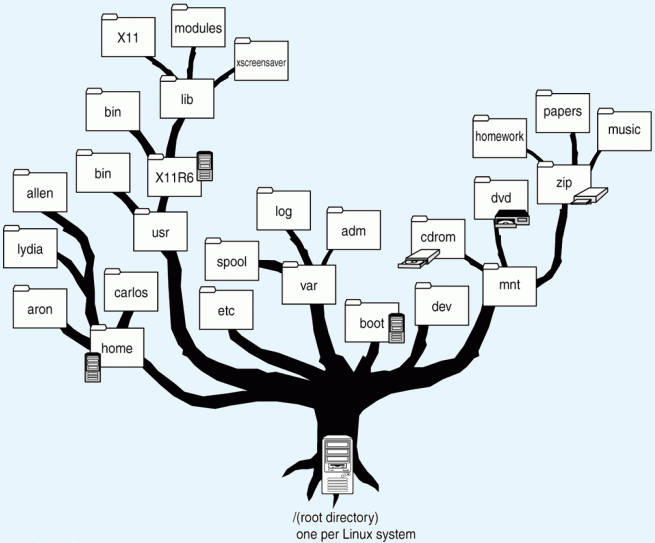
\includegraphics[height=7cm]{img/estructura.jpg}
\end{figure}
\end{frame}

\begin{frame}{Directorios principales}
\begin{itemize}
\item \textbf{/ :} es el nivel más alto dentro de la jerarquía de directorios.
\item \textbf{/bin:} aplicaciones binarias de comandos esenciales para una sesión de usuario único o mutliusuario (Incluyen por ejemplo cat, ls, cp, rm, etc).
\item \textbf{/sbin: }sistema de binarios esencial, comandos y programas exclusivos del superusuario (Por ejemplo init, route, ifup).
\item \textbf{/dev:} permite interactuar con los dispositivos del equipo.
\item \textbf{/etc:} archivos de configuración del sistema específico del Host de todo el sistema. 
\item \textbf{/home:} carpeta por defecto de los usuarios.
\item \textbf{/tmp:} almacena ficheros temporales.
\item \textbf{/root:} directorio home del usuario root. 
\item \textbf{/mnt:} sistema de archivos montados temporalmente. Discos duros y particiones de forma temporal en el sistema.
\end{itemize}
\end{frame}
\begin{frame}{Instalación}
\begin{multicols}{2}
\centering
\begin{figure}
	
\includegraphics[height=3cm]{img/rhel.png}
\end{figure}
\textbf{Red Hat} Enterprise Linux 7.4
\begin{figure}
	
\includegraphics[height=3cm]{img/Virtualbox.png}
\end{figure}
\textbf{ \href{https://download.virtualbox.org/virtualbox/6.0.4/VirtualBox-6.0.4-128413-Win.exe}{Oracle VirtualBox}}

\end{multicols}

\end{frame}
\subsection{Comandos básicos para administración de archivos y directorios}
\begin{frame}{Editores de texto}
\textbf{Editor Vi:} \\editor de texto que maneja en memoria el texto entero de un archivo.\\[0.5cm]
\textbf{Inicio Vi:} 
\begin{center}
\boxed{\texttt{\$ vi \textit{file}}}
\end{center}
Abre el archivo \textit{file}, en caso de no existir, abre el editor como si existiera.\\[0.5cm]
\textbf{Modos de Vi}
\begin{itemize}
    \item Comando
    \item Inserción
    \item Línea
\end{itemize}
\end{frame}
\begin{frame}{Modos de Vi}
\textbf{Modo Comando} \textit{\small (Case Sensitive)}\\[0.5cm]
{\scriptsize
\begin{tabular}{l|p{8cm}}
     \textsc{Comando}&\textsc{Acción}\\\hline
     Flechas / \texttt{H,J,K,L} & Desplazamiento: Izquierda, Abajo, Arriba, Derecha.\\\hline
     \textbf{X}\texttt{G} & Ubicarse en el número de línea \textbf{X} del archivo.\\\hline
     \texttt{i} / \texttt{I} & Cambiar a modo insertar: a la izquierda del cursor/al comienzo de la línea del cursor.\\\hline
     \texttt{x} &Borrar caracter debajo del cursor.\\\hline
     \textbf{X}\texttt{dd} &Borrar las próximas \textbf{X}  debajo del cursor.\\\hline
     \textbf{X}\texttt{yy} &Copiar las siguientes \textbf{X} líneas debajo del cursor. \\\hline
     \texttt{p} &Pegar el contenido debajo del cursor. \\\hline
     \texttt{u} &Deshacer último cambio realizado.
\end{tabular}

}
\end{frame}
\begin{frame}
\textbf{Modo Inserción}\\
Se ingresa el texto deseado, para salir de este modo se lo hace con la tecla \texttt{ESC}.\\[0.5cm]
\textbf{Modo Línea}\\
Se ingresa a ese modo con las teclas.
{\scriptsize
\begin{tabular}{l|l}
\textsc{Comando}&\textsc{Acción}  \\\hline
/\textbf{texto} & Busca hacia adelante la cadena de caracteres \textbf{texto}.\\\hline
?\textbf{texto} & Busca hacia atrás la cadena de caracteres \textbf{texto}.\\\hline
:q & Salir si no hubo cambios. \\\hline
:q! & Salir sin guardar cambios.\\\hline
:w \textit{archivo01} & Guardar cambios. \textit{Se guarda con el nombre archivo01}.\\\hline
:wq & Guardar cambios y salir.

\end{tabular}
}
\end{frame}
\begin{frame}{Práctica Vi}
\begin{itemize}
    \item Abrir un documento con el nombre de \texttt{fileSUD.txt} y escribir la siguiente línea:
    \begin{center}
        \texttt{Esta es la línea numero uno.}
    \end{center}
    \item Desde comando copiar 9 veces la línea escrita y pegarla debajo de la misma. En el modo inserción editar cada línea con el número correspondiente.
    \item Desde comando, copiar cada línea el número de veces que represente la línea, hasta la línea número cinco.
\end{itemize}
\end{frame}
\begin{frame}{fileSUD.txt}
\lstinputlisting{files/fileEJ.txt}
\end{frame}

\begin{frame}{fileSUD.txt}

\lstinputlisting{files/fileEJ2.txt}

\end{frame}
\begin{frame}{Comandos básicos para administración de archivos}
\begin{itemize}
    \item El intérprete de comandos es \textit{}{case-sensitive}.
\end{itemize}
{\scriptsize
\begin{tabular}{c|p{6cm}|l}
\hline
\textbf{clear} & Borra la pantalla   &\\
\textbf{more}  & Visualiza archivos en páginas  & \texttt{more /etc/redhat-release}\\
\textbf{pwd} & Visualiza la ubicación del directorio actual   &\\
\textbf{ls} & Muestra un listado de los archivos y directorios de un directorio   & \texttt{ls -la \textit{directorio} }\\
\textbf{rm} & Eliminar archivos   & \texttt{rm -r -f  \textit{nombreArchivo}}\\
\textbf{cd} & Cambiar de directorio   & \texttt{cd} \\
\textbf{mkdir} & Crea directorio   & \texttt{mkdir /tmp/directorio} 
\end{tabular}
 }   
\end{frame}
\subsection{Gestión y administración de usuarios y grupos}
\subsection{Gestión, administración e instalación de procesos/paquetes RPM}
\subsection{Empaquetado y compresión de archivos y directorios}
%meter aqui TIPO DE SISTEMAS DE FICHEROS con compresion y eso
\section{Módulo 2}


% \subsection{Tables and Figures}

% \begin{frame}{Tables and Figures}

% \begin{itemize}
% \item Use \texttt{tabular} for basic tables --- see Table~\ref{tab:widgets}, for example.
% \item You can upload a figure (JPEG, PNG or PDF) using the files menu.
% \item To include it in your document, use the \texttt{includegraphics} command (see the comment below in the source code).
% \end{itemize}

% Commands to include a figure:
%\begin{figure}
%\includegraphics[width=\textwidth]{your-figure's-file-name}
%\caption{\label{fig:your-figure}Caption goes here.}
%\end{figure}

% \begin{table}
% \centering
% \begin{tabular}{l|r}
% Item & Quantity \\\hline
% Widgets & 42 \\
% Gadgets & 13
% \end{tabular}
% \caption{\label{tab:widgets}An example table.}
% \end{table}

% \end{frame}

% \subsection{Mathematics}

% \begin{frame}{Readable Mathematics}

% Let $X_1, X_2, \ldots, X_n$ be a sequence of independent and identically distributed random variables with $\text{E}[X_i] = \mu$ and $\text{Var}[X_i] = \sigma^2 < \infty$, and let
% $$S_n = \frac{X_1 + X_2 + \cdots + X_n}{n}
%       = \frac{1}{n}\sum_{i}^{n} X_i$$
% denote their mean. Then as $n$ approaches infinity, the random variables $\sqrt{n}(S_n - \mu)$ converge in distribution to a normal $\mathcal{N}(0, \sigma^2)$.

% \end{frame}

\section{Módulo 3}


\end{document}
